\chapter{Proyecto}

\section{Introduccion}
En este proyecto se pretende desarrollar una aplicacion web de tipo economia colaborativa, en la que se gestionen los parqueaderos en la ciudad y los usuarios puedan solicitar un servicio de alquiler de los mismos, de igual manera, los mismos usuarios pueden ofrecer en alquiler un parqueadero en su propiedad, todo basandose en, como se menciono antes, un consumo colaborativo, en el cual los consumidores pueden actuar como proveedores de recursos o receptores de recursos.



\newpage
\section{Descripción General}
La plataforma esta pensada para generar un comercio virtual entre arrendatario/arrendador de manera simple y practica, para poder alquilar u ofrecer en alquiler un espacio donde aparcar cualquier tipo de vehiculo, ya sean carros, camionetas, motos, e incluso bicicletas y vehiculos especiales, todo funcionando como una economia colaborativa donde cualquier persona pueda obtener un beneficio al usar la plataforma, se va a utlizar un sistema de valoraciones tanto para quien ofrece un espacio como para quien decide tomar éste en alquiler, todo a manera de guia para los usuarios.

\newpage
\section{Objetivos}
El proyecto tiene como objetivo principal facilitar el transporte en la ciudad para usuarios de carros, motos, bicicletas, etc. sin tener que preocuparse por donde van a estacionar su vehiculo o por el precio que van a pagar, esto con el afan de agilizar y facilitar el proceso de apartado de un espacio para aparcar un vehiculo, ademas de combatir los arbitrarios precios de parqueaderos en sectores de mucha consentracion laboral o estudiantil.

\newpage
\section{Alcances y Limites}
\large \textbf{Alcances}  \\
\\
El presente proyecto explorara el sector vehicular en la ciudad, apuntando sobretodo, al sector de la poblacion que se presenta constantemente a espacios donde se pagan unos muy altos precios de estacionamiento, o donde es muy limitado el espacio para aparcar, ya sea una zona de alta densidad laboral, cerca a un centro comercial, o una zona universitaria.
\\
\\
\large \textbf{Limites}  \\
\\
Las limitaciones del proyecto van mas orientadas a los sectores donde el sistema de parqueo no presente fallos criticos, es decir, sectores con baja concurrencia vehicular no se contemplan dentro del proyecto por su baja probabilidad tanto de potenciales arrendatarios como de potenciales arrendadores, aunque esto va directamente ligado al desarrollo del proyecto. 
\newpage

\section{Cronograma}
\begin{figure}[h!]
	\centering
	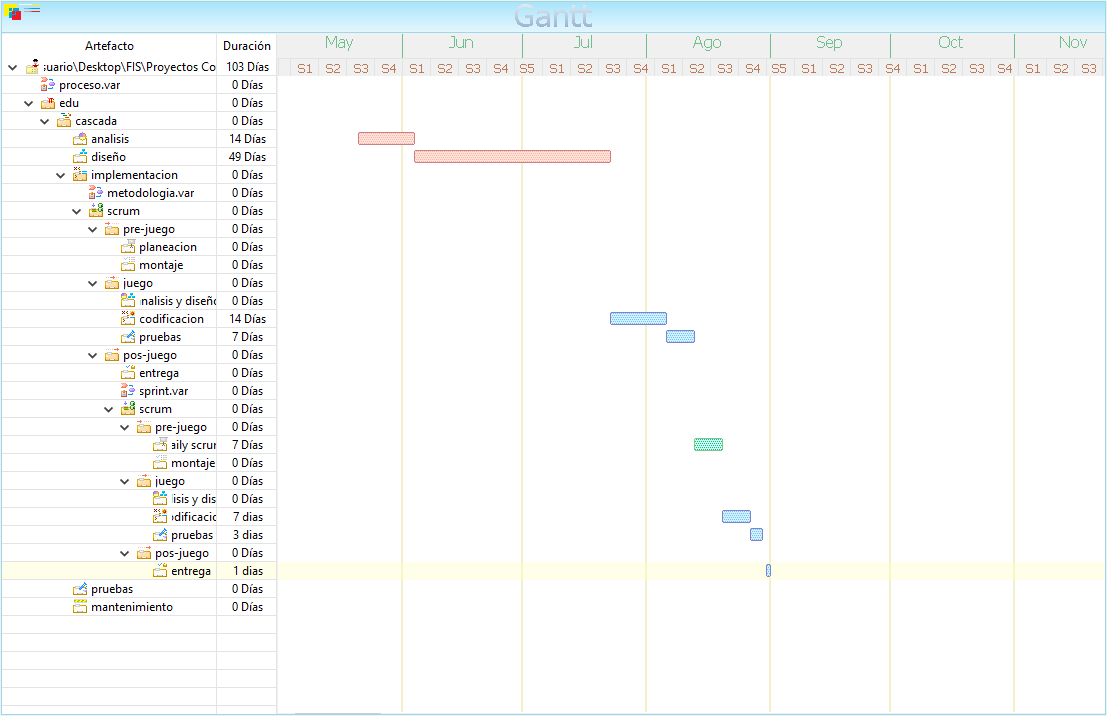
\includegraphics[width=1.1\linewidth]{imgs/CronogramaColoso.png}
	\caption[Cronograma]{TimeLine del Cronograma}
\end{figure}

\large \textbf{Descripcion}  \\
\\
El Cronograma consta de una duracion de aproximadamente 14 semanas donde se hace un especial enfasis en la etapa de diseño, correspondiente al proceso que vamos a incorporar (Modelo de Cascada) se debe enfocar una gran parte de los esfuerzos del equipo en esta etapa de diseño, esto, despues de haber realizado el correspondiente analisis de requerimientos, con todo lo que conlleva esta etapa.
\\
\\
Una vez finalizada de etapa de diseño, se incorpora una metodologia agilista para enfrentar la etapa de implementacion, la Metodologia SCRUM, donde unicamente tomamos de esta metodologia, como ya se menciono, la fase de implementacion y prueba, que consta de dos iteraciones del proceso tanto de codificacion como de sus respectivas pruebas, este proceso en total suele llevar entre 2 a 4 semanas, donde en este periodo, ademas de realizar los procesos ya mencionados, internamente contiene una fase de daily Scrum, cuya finalidad es relizar reuniones diarias para retroalimentar el trabajo hasta ese punto, ver los posibles fallos y compartir las ideas del equipo, tal y como lo describe el modelo.
\\
\\
Y para finalizar, con los timpos justos del semestre y esperando que no haya ningun tipo de contratiempo, se espera realizar la correspondiente entrega del proyecto.
\newpage